\chapter{Политика}


\section{20 лет Владимира Путина: трансформация режима}

\textit{Политолог Кирилл Рогов открывает цикл статей о том, как изменилась страна за путинские годы}

\textit{Источник: \url{www.vedomosti.ru/opinion/articles/2019/08/07/808337-20-let-putina}}

\textit{Кирилл Рогов }

20 лет назад Владимир Путин внезапно появился на политическом олимпе в образе эффективного бюрократа с силовым бэкграундом, рыночно ориентированного государственника и прагматика, чуждого идеологических пафосов. Сегодня Путин выглядит сильным авторитарным лидером (типаж «стронгмен»), увлеченным геополитическим противостоянием с Западом и идейной борьбой с мировым либерализмом, решительно жертвующим ради этого прагматическими целями развития страны. И даже когда он заговаривает о модернизации, разговор довольно быстро сбивается на виды вооружений.

\textbf{Две эпохи}



Если бы Путин ушел в 2008 г., то остался бы в истории как один из самых успешных лидеров России. После 15 лет кризисов и пертурбаций в стране наступила относительная стабилизация на условиях «управляемой демократии» (что бы это ни значило), но главное – начался период интенсивного экономического роста (7% в год в среднем) и еще более впечатляющий рост душевых доходов.

Конечно, недоброжелатели говорили бы, что причина успехов – это восстановительная фаза трансформационного цикла и рост цен на нефть. И, разумеется, в шкафах этого успешного правления уже к тому моменту скопилось немало скелетов: вторая чеченская война и ее последствия, дело ЮКОСа, создание правовых и хозяйственных гибридов в виде госкорпораций и еще кое-что. Но все это не смогло бы в исторической памяти перевесить той атмосферы успеха, на волне которой Путин покинул бы свой пост.

Вторая часть путинского двадцатилетия (2009–2019 гг.) была в значительной мере противоположна первой. Два экономических кризиса, связанных с волатильностью цен на нефть (2009 и 2015 гг.); политический кризис, вызванный московскими протестами 2011–2012 гг. и развернувший режим в сторону авторитарного ужесточения, доминирования силовых элит и их логик при принятии решений. Это последнее обстоятельство создало спусковой механизм следующего кризиса – внешнеполитического, связанного с аннексией Крыма и войной на Восточной Украине. Принятые тогда решения не были вынужденными и единственно возможными. Но эти решения, сделавшие конфронтацию с Западом основной рамкой жизни страны, окончательно закрепляли доминирование силовых элит и силовых логик во всех сферах государственной жизни.

Итак, череда экономических, внутри- и внешнеполитических кризисов (2008–2009, 2011–2012, 2014–2015 гг.), а также три войны (Грузия, Украина и Сирия) формируют основную сюжетную канву второй части путинского правления. При этом среднегодовые темпы роста упали до 0,6\% в год. В итоге в 2000 г. ВВП на душу населения в России составлял 14,5\% от уровня США и 21,5\% от уровня стран ЕС, в 2008 г. это было соответственно 22,5 и 32\%, а в 2018 г. – 21,5 и 31\%. Это и есть стагнация – неспособность сокращать разрыв с лидерами (при том что среднегодовая цена на нефть в первом периоде составила \$54 за баррель, а во втором – \$74).

\textbf{Тотальный ревизионизм}



Путин не просто не ушел в 2008 г. На самом деле в моменте неухода решительно менялось его целеполагание. В 2000 г. он пришел со сверхзадачей стабилизации и деполитизированной модернизации, выполнения которой и добивался теми способами, которые были ему в силу его компетенций доступны. Во втором периоде его сверхзадачей стало пересоздание той государственно-политической системы (несомненно, весьма лабильной и гибридной), которая складывалась по итогам первого постсоветского десятилетия.

С этим связан тотальный путинский ревизионизм второго периода: абсолютизация понятия «суверенитет», поиски новых опор в виде «скреп» и «традиционных ценностей», вытесняющих императивы модернизации, конструирование «национально ориентированных элит», фактический отказ от признания границ, сложившихся по итогам распада СССР, и решительный разворот от сотрудничества к конфронтации в отношениях с Западом.

Возможно, все это имело бы больший успех, если бы формирующаяся путинская система демонстрировала экономическую эффективность хотя бы в той мере, в какой это удавалось авторитарному Казахстану (ВВП на душу населения там в 2000 г. составлял 10\% от американского, в 2008 г. – 18\%, а в 2018 г. – 20,5\%, почти сравнявшись с российским). Но она этого сделать не смогла. И даже ее некоторые успехи в построении «эффективного авторитаризма» в отдельных сферах госуправления не могут компенсировать этого фундаментального факта.

В итоге новое целеполагание превращается в голую проповедь антилиберализма и антизападничества, переосмысление «границ русского мира» – в формирование пояса конфронтации и недоверия вокруг России, а конструирование «национально ориентированных элит» – в безраздельное господство силовиков и силовых олигархий, постоянно требующих льгот, преференций и денежных вливаний.

\textbf{Откуда и куда}



Эволюция политического режима постсоветской России может быть описана в терминах сравнительной политологии следующим образом. Режим, сложившийся к концу первого постсоветского десятилетия, можно охарактеризовать как конкурентную олигархию. Это режим, сочетающий достаточно высокую конкурентность в публичной сфере с одной стороны, и слабый, коррумпированный правопорядок – с другой. Такие режимы и сейчас существуют на Украине, в Молдавии, Киргизии и ряде стран Латинской Америки.

Путинская стабилизация 2000-х гг. и экономический рост, сопряженный с быстрым ростом рентных доходов казны, сформировали в России тип режима, который обычно называют «конкурентным авторитаризмом». В таком режиме правящая коалиция резко ограничивает возможности политической конкуренции, свободу СМИ, опираясь в том числе на достаточно широкую, но пассивную поддержку «снизу», которая (в свою очередь) обеспечена убедительной экономической динамикой. При том что правящая коалиция надежно держит власть в руках (используя в том числе административные рычаги и фальсификации на выборах), оппозиция здесь вполне легитимна, располагает определенной инфраструктурой и поддержкой граждан и элитных групп.

Авторитарный лидер или правящая партия обычно получают на выборах результат в диапазоне 60–70\%, который и демонстрирует, что примерно треть населения голосует против режима, но такое поведение считается легитимным и не угрожает его стабильности. И самое важное – эти режимы низкорепрессивные. За исключением отдельных случаев, им достаточно административных мер, чтобы секьюритизировать свое доминирование.

Такой режим существовал в путинской России примерно с 2003 по 2012 г. Политический кризис 2011–2012 гг. обозначил его закат. Однако важно подчеркнуть, что не выступления оппозиции привели к этому, а скорее экономический кризис 2008–2009 гг., подорвавший доверие граждан к режиму, что и проявилось в их реакции на фальсификацию результатов парламентских выборов в 2011 г. (в 2008 г. соизмеримые фальсификации не вызывали ни малейшего возмущения).

\begin{wrapfigure}{r}{0.7\textwidth}
    \begin{center}
        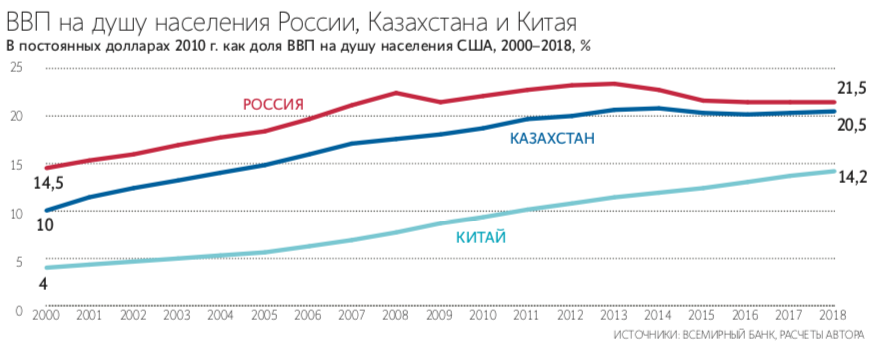
\includegraphics[width=0.68\textwidth]{img/1tbz.png}
    \end{center}
\end{wrapfigure}
\textbf{Авторитарный дедлок.} Более жесткие деспотические режимы политологи называют «авторитарной гегемонией». На выборах здесь авторитарный лидер или правящая партия регулярно получают от 75 до 99\% голосов. Что, однако, свидетельствует не об их популярности, а о том, что они оказывают гораздо более систематическое давление на оппозицию, независимые СМИ и нелояльные элитные группы, т. е. отличаются от предыдущего типа резко возрастающим уровнем репрессивности. Встречаются они сегодня почти исключительно в Азии, Африке и бывшем СССР.

Как показывает опыт ряда азиатских стран, эволюция режима от первого типа ко второму часто происходит на фоне ухудшения экономической динамики. По мере того как экономика играет все меньшую роль в обеспечении легитимности и устойчивости режима, все большую роль начинают играть две другие опоры: репрессии и идеология. В информационной политике режим переходит от фильтрации и ограничения информации к агрессивной пропаганде. Начинаются систематические преследования гражданского активизма, появляются нормы, позволяющие в уголовном порядке преследовать за слова, криминализуется уличная активность граждан.

Именно переход от режима конкурентного авторитаризма к авторитарной гегемонии составил политическое содержание последнего путинского периода – с 2013 по 2019 г. А геополитическая конфронтация выступила в качестве той идеологической рамки, которая легитимирует возрастающую репрессивность.

Хотя Россия выглядит сегодня гораздо более авторитарной страной, чем в 2012 г., этот переход, видимо, следует считать пока незавершенным. Наверное, играют свою роль развитая социальная инфраструктура мегаполисов, уровень европеизированности элит, глубина проникновения интернета и социальных медиа. Ну, и разумеется, экономический застой. Несмотря на это, Путин вряд ли оставит свои усилия по девестернизации России. И это бесплодное (в исторической перспективе) перетягивание каната скорее всего останется главным сюжетом финальной фазы его политической карьеры.


